\documentclass[tikz]{standalone}
\begin{document}

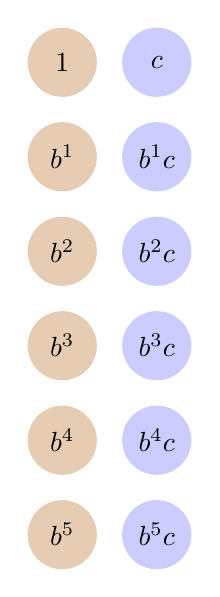
\begin{tikzpicture}
\newcommand{\Radx}{1.2}
        \foreach \x in {1,...,5} { %60,120,...,359} {
                \node[circle,minimum size=2.5em,fill=blue!20] at (1.2,{-\Radx*\x}) {\(b^{\x}c\)};
                \node[circle,minimum size=2.5em,fill=brown!40] at (0,{-\Radx*\x}) {\(b^{\x}\)};
		}
        \node[circle,minimum size=2.5em,fill=blue!20] at (1.2,0) {\(c\)};
        \node[circle,minimum size=2.5em,fill=brown!40] at (0,0) {\(1\)};        
\end{tikzpicture}
\end{document}
